\subsubsection{Backend erstellen}
Das Backend umfasst alle Funktionen, welche vom Benutzer nicht gesehen werden können. Diese bearbeitet den Datentransfer, Datenaufbereitung und die Datensicherheit.
\paragraph{Aktivitätsdiagramm Backend}\mbox{}\\
\begin{figure}[H]
	\centering
	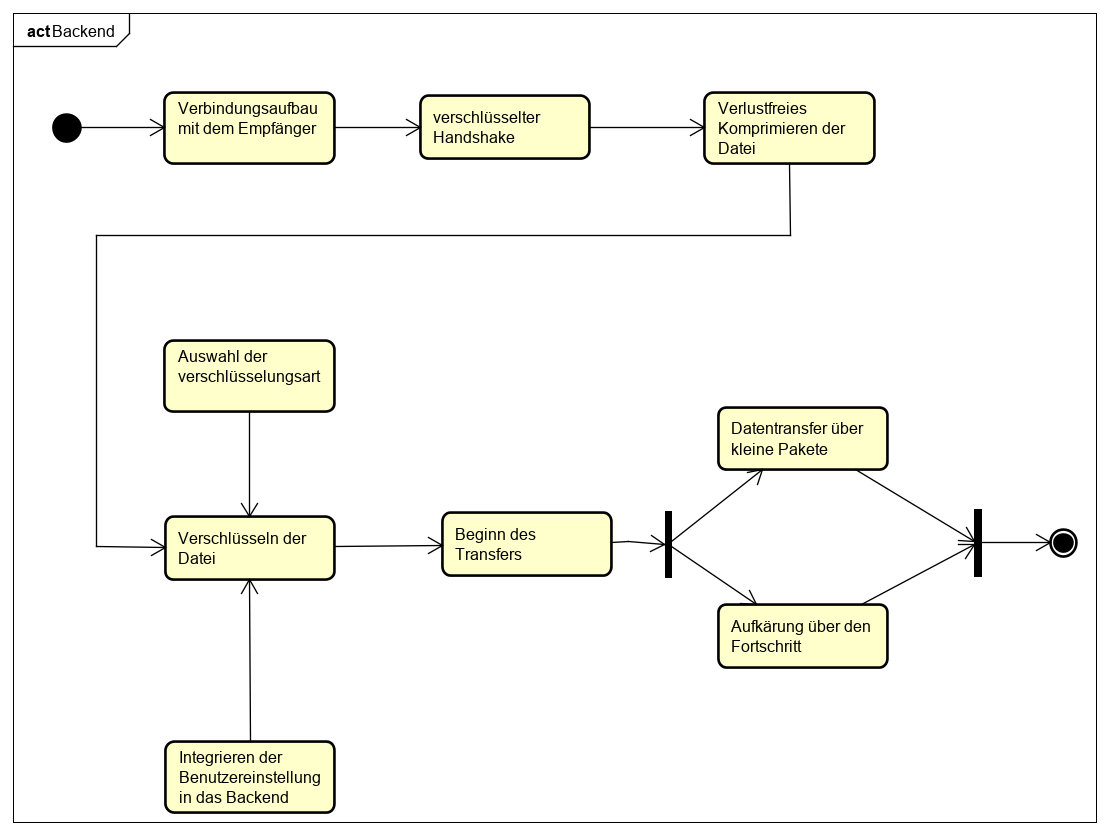
\includegraphics[width= 0.9\linewidth]{diagramms/activity/Backend.png}
	\caption{Aktivitätsdiagramm Backend}
\end{figure}
\newpage
\begin{indentE}\mbox{}
	\paragraph{/LF1110/ Verbindung aufbauen}\mbox{}\\
	Es wird die Verbindung mit dem ausgewählten Empfänger aufgebaut. Dieser Verbindungsaufbau besteht aus einem verschlüsselten Handshake, mit welchem die Systemdaten des Empfängers und Senders ausgetauscht werden. Wenn Empfänger und Sender den selben Verschlüsselungsschlüssel gewählt haben, ist der Handshake erfolgreich und der Transfer kann beginnen.
	\UseCase{
		{Desktop Backend}
		{/LF1110/ Verbindung aufbauen}
		{Backend}
		{Es wird die Verbindung mit dem Empfänger als Sender aufgebaut.}
		{Es muss eine Verbindung zwischen Empfänger und Sender für den Datentransfer herrschen}
		{Der Empfänger kann sich mit einem Empfänger der Wahl verbinden.}
		{Empfänger, Sender}
		{Sender, Namen }
		{Der Sender kann sich nicht mit dem Empfänger verbinden.}
		{Der Sender kann sich mit dem Empfänger verbinden.}
		{hoch}
		{mittel}
		{Must Have}
	}
	\paragraph{/LF1120/ Daten transferieren}\mbox{}\\
	Die Daten werden in kleinen Paketen versandt, um die Datensicherheit zu garantieren. Dabei haben diese eine einheitliche Größe und es werden unterschiedliche viele je nach Datengröße versandt. Dabei sollen der Empfänger und der Sender um den Fortschritt der Übertragung aufgeklärt werden.
	\UseCase{
		{Desktop Backend}
		{/LF1120/ Daten transferieren}
		{Backend}
		{Die Daten sollen vom Sender zum Empfänger transferiert werden. Diese soll dabei möglichst verlustlos gesendet werden.}
		{Der Daten müssen an den Empfänger gebracht werden.}
		{Die Daten des Sender kommen beim Empfänger an.}
		{Empfänger, Sender}
		{Datei(Name, Größe, Inhalt), Fortschritt(aus index und Anzahl Pakete), Sender, Empfänger}
		{Die Daten können dem Empfänger nicht vom Sender geschickt werden.}
		{Die Daten werden vom Sender zum Empfänger verlustlos gesendet.}
		{hoch}
		{gering}
		{Must Have}
	}
	\paragraph{/LF1130/ Daten komprimieren}\mbox{}\\
	Die Daten werden vor dem Versand verlustlos komprimiert, um die Datenmenge zu verkleinern. Die dabei gewählt Komprimierungsart, darf vom Auftragnehmer ausgewählt werden.
	\UseCase{
		{Desktop Backend}
		{/LF1130/ Daten komprimieren}
		{Backend}
		{Die Daten sollen vor dem Transfer verlustlos komprimiert werden, um die Übertragungsdauer zu verringern}
		{Der Datentransfer soll kürzer dauern.}
		{Der Datentransfer dauert in den meisten Fällen kürzer.}
		{Sender, Empfänger}
		{Daten}
		{Die Datenübertragung dauert länger.}
		{Die Datenübertragung dauert kürzer.}
		{mittel}
		{mittel}
		{Should Have}
	}
	\paragraph{/LF1140/ Datentransfer verschlüsseln}\mbox{}\\
	Der Datentransfer wird mit einem Verschlüsselungsschlüssel nach dem AES256 Standard verschlüsselt, um die Datensicherheit zu erhöhen. Diese wird dann vom Empfänger wieder entschlüsselt. Die dafür benutzte Verschlüsselungsart, kann vom Auftraggeber ausgewählt werden.
	\UseCase{
		{Desktop Backend}
		{/LF1140/ Datentransfer verschlüsseln}
		{Backend}
		{Der Datentransfer soll für eine höhere Sicherheit durch einen Schlüssel verschlüsselt werden.}
		{Der Datentransfer soll verschlüsselt stattfinden, damit die originalen Daten nicht von Dritten ausgelesen werden können.}
		{Der Datentransfer erfüllt den Standard AES256.}
		{Empfänger, Sender, Dritte}
		{Daten, Schlüssel}
		{Die originalen Daten können von Dritten ausgelesen werden}
		{Die originalen Daten sind während dem Transfer verschlüsselt}
		{mittel}
		{mittel}
		{Must Have}
	}
	\paragraph{/LF1150/ Benutzereinstellungen integrieren}\mbox{}\\
	Die vom Benutzer ausgewählten Benutzereinstellungen müssen in das Backend integrierte werden, um den Nutzen aus diesen Werten zu ziehen.
	\UseCase{
		{Desktop Backend}
		{/LF1150/ Benutzereinstellungen integrieren}
		{Backend}
		{Die Benutzereinstellungen sollen integriert werden.}
		{Die ausgewählten Benutzereinstellungen sollen in das Backend integriert werden.}
		{Die Einstellungen des Benutzer haben eine Auswirkung auf das Backend.}
		{Sender, Empfänger}
		{gewünschte Systemname, Verschlüsselung (Ja/Nein), Standardschlüssel, Speicherort}
		{Der Benutzer muss die meisten Daten bei jeder Übertragung neu einstellen, wodurch diese länger dauert}
		{Der Übertragung ist anpassbar, wodurch diese verschnellert werden kann. }
		{mittel}
		{gering}
		{Should Have}
	}
\end{indentE}